\documentclass[11pt]{article}
\usepackage{fullpage}
\usepackage{setspace}
\usepackage{amsmath}
\usepackage{fancyvrb}
\usepackage{enumerate}
\usepackage{pgfplots}
\usepackage{graphicx}
\usepackage{float}
\usepackage{multirow}
\usepackage[format=hang,labelsep=quad]{caption}
\usepackage{subfig}
\usepackage{array}
\usepackage{multirow}

\renewcommand\thesubfigure{\roman{subfigure}}


\begin{document}
\noindent\large{Math 5365}\\
\large{Data Mining 1}\\
\large{Homework 19}\\
\large{Mary Barker}
\doublespace
\begin{enumerate}
\item 
 Test whether the k-means clusters for the wdbc data set are 
 statisticaly independent of Diagnosis using a chi-square test with 
 a simulated p-value.

$\chi^2$ test with simulate.p.value = T
\begin{Verbatim}
	Pearson's Chi-squared test with simulated p-value (based on 2000
	replicates)

data:  wdbc_tab
X-squared = 279.65, df = NA, p-value = 0.0004998
\end{Verbatim}

The p-value is significantly smaller than 0.05, so the clusters 
\textit{are} dependent.

\item
 In this problem, you will apply the DBSCAN clustering method on the 
 wdbc data. 

\begin{enumerate}
\item 
 Create a plot of sorted k-dist values, where k = 5, and determine 
 the optimal vlaue of Eps. 

%This is with Eps = 4.35
%\begin{center}
%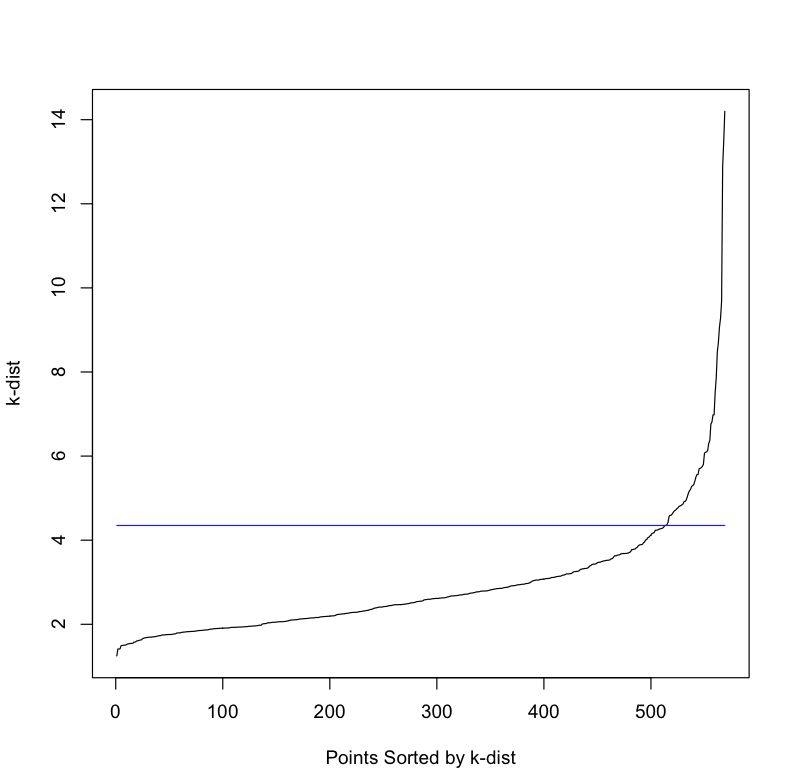
\includegraphics[scale=0.35]{pix/k_dist}
%\end{center}

The optimal value for Eps is approximated as 3.75, as shown in the graph below.
%This is with Eps = 3.75
\begin{center}
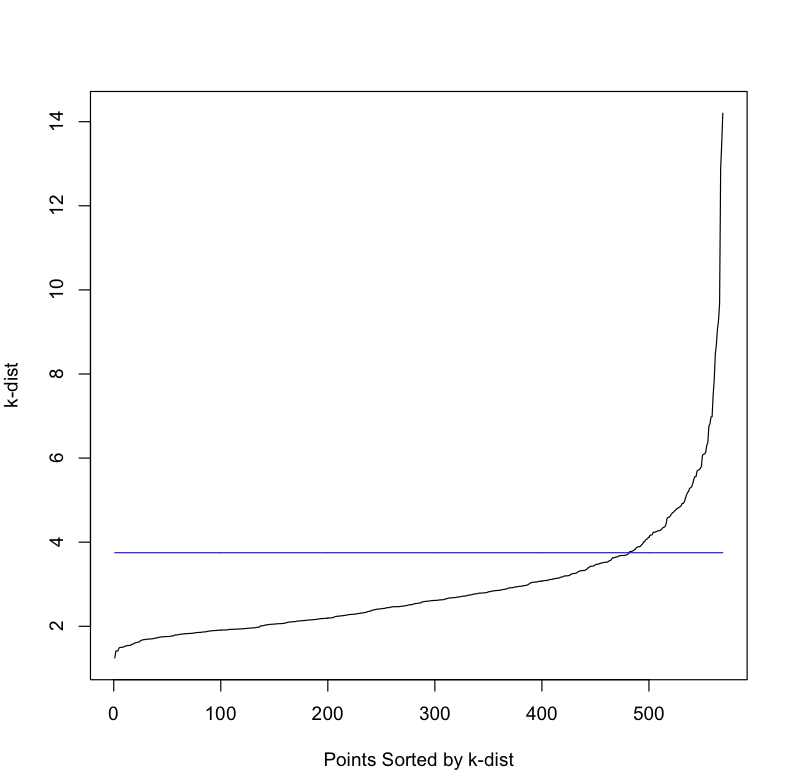
\includegraphics[scale=0.35]{pix/k_dist1}
\end{center}

\item
 Perform DBSCAN using this value of Eps and k = 5
%Eps = 4.35: 
%The table for this is shown below:
%
%\begin{center}
%\begin{tabular}{c c c}
%  & predicted & \\
%    &  B  &  M \\
%  B & 343 &  14 \\
%  M & 190 &  22 \\
%\end{tabular}
%\end{center}
%
%Eps = 3.75:
%The table for this is shown below:
The confusion matrix for the DBSCAN model is shown below. 

\begin{center}
\begin{tabular}{c c c}
  & predicted & \\
    &  B  &  M \\
  B & 334 &  23 \\
  M & 174 &  38 \\
\end{tabular}
\end{center}

\item How many clusters were identified? 

There were only two values for \verb|wdbc_dbscan|, 0 and 1. Therefore there was only 
1 cluster. 

\item What percentage of the points in the data were classified as noise? 

about 6.326889 \% 

\item
 Test whether the dbscan clusters are statistically independent of 
 Diagnosis using a chi-square test with a simulated p-value. 

The output for the $\chi^2$ test is shown below.
\begin{Verbatim}

	Pearson's Chi-squared test with simulated p-value (based on 2000
	replicates)

data:  wdbc_tab
X-squared = 9.3537, df = NA, p-value = 0.002499
\end{Verbatim}
Note that the p-value is much smaller than 0.05. Thus the cluster is 
most likely not independent of Diagnosis. 

\end{enumerate}

\end{enumerate}

\begin{Verbatim}
#Data Mining hw 19
library(stats)
library(cluster)
library(fields)
library(fpc)

source('~/Dropbox/Tarleton/data_mining/generic_functions/dataset_ops.R')
wdbc <- read.csv('~/Dropbox/Tarleton/data_mining/dfiles/wdbc.data',
                 header=F,sep=',')
wdbc <- wdbc[,-1]
nr <- nrow(wdbc) 
nc <- ncol(wdbc) 

# 1 Test whether the k-means clusters for the wdbc data set are 
#   statisticaly independent of Diagnosis using a chi-square test with 
#   a simulated p-value.

wdbc_kmeans <- kmeans_reps(wdbc[2:nc], 2, 1000)
predicted <- rep('',nr)
predicted[1 * (wdbc_kmeans$cluster == 2) == 1] <- 'B'
predicted[1 * (wdbc_kmeans$cluster == 1) == 1] <- 'M'
wdbc_tab <- table(wdbc$V2, predicted)

chisq.test(wdbc_tab, simulate.p.value = T)
chisq.test(wdbc_tab, simulate.p.value = F)

# 2 In this problem, you will apply the DBSCAN clustering method on the 
#   wdbc data. 

#  a. Create a plot of sorted k-dist values, where k = 5, and determine 
#     the optimal vlaue of Eps. 

k = 5
z <- standardize(wdbc, 2:nc)
dmat <- rdist(z[,2:nc])

sort_dmat <- apply(dmat, 2, sort)
kdist <- sort_dmat[k,]
plot(sort(kdist), type='l', 
     xlab = 'Points Sorted by k-dist', 
     ylab = 'k-dist')
lines(1:length(kdist), rep(3.75, length(kdist)), col='blue')
#lines(1:length(kdist), rep(4.35, length(kdist)), col='blue')

#myEps = 4.35
myEps = 3.75
#  b. Perform DBSCAN using this value of Eps and k = 5

wdbc_dbscan <- dbscan(z[,2:nc], eps = myEps, MinPts = k)
plot(z[,2], z[,8], col = (wdbc_dbscan$cluster + 1))

predicted <- rep('',nr)
predicted[1 * (wdbc_dbscan$cluster == 1) == 1] <- 'B'
predicted[1 * (wdbc_dbscan$cluster == 0) == 1] <- 'M'
wdbc_tab <- table(wdbc$V2, predicted)

#  c. How many clusters were identified? 

#  d. What percentage of the points in the data were classified as noise? 

#  e. Test whether the dbscan clusters are statistically independent of 
#     Diagnosis using a chi-square test with a simulated p-value. 

chisq.test(wdbc_tab, simulate.p.value=T)
\end{Verbatim}
\end{document}
